\documentclass[]{scrartcl}

\usepackage{url}
\usepackage{graphicx}

%opening
\title{Testing Containers in the Cloud}
\author{Florian Hofer}
\date{}

\begin{document}

\maketitle

\begin{abstract}
	This document contains a global summary of steps taken, test done and options reviewed for the concept of application containerization under real-time constrains in the cloud. To better follow the execution order, chapters are listed in chronological order indicating approximate time values.
\end{abstract}

\section{Introduction}



Virtualbox >5.x with extension pack is needed

\section{System Tests and variants}

{\small\textsc{Identification of application candidates, 25-30/07/18} \bigskip}

Before selecting a specific setup, different variants of systems are tested for their real-time capabilities, maintainability and ease of setup. Candidates for this session are:

\begin{itemize}
	\item \textbf{resinOS} operating system designed to run containers on different architectures and hardware devices
	\item \textbf{ubuntu Core} an operating system for IoT devices implemented using the new snap image approach
	\item \textbf{Xenomai 3} the co-core extension for Linux based operating systems, which allows hard-real-time scheduling
	\item \textbf{PREEMPT\_RT} a kernel patch for linux based systems incrementing the preemption level for soft-realtime based
	\item \textbf{CGroups} resource partitioning and CPU pinning (affinity selection), also in combination with previous system.
\end{itemize}

The systems are setup in virtual machines and verified for real-time scheduling properties. Installations verify runtime of containers of different type, including synthetic applications.

\subsection{resinOS by Resin.io}

{\small\textsc{Testrun resinOS, 25/07/18} \bigskip}

\textit{resinOS} is an Project-Yocto based operating system designed by ``resin.io'' for containerized running of small systems. The design also includes a cloud based monitoring system where the connect to. The images and deltas of containers are also managed via a Balena engine on the \texttt{resin.io} website. The containers supplied by resinOS are based on the lightweight general purpose Alpine Linux.




\subsubsection{Local Virtual Machine}

The resinOS operating system was primarily made to run on low resource systems, embedded devices or alike, and does thus not have a specific image for desktop/laptop or server. To run the OS in a virtual machine we download the Intel based 64 bit image for the Intel NCU from the resinOS website. \url{https://resinos.io/#downloads}

The image does not contain any additional configuration concerning network setup or ssh keys to be able to connect to the device. To configure the image, we need the CLI tool. Before installing the tool, make sure that following packages are installed:

\begin{itemize}
	
	\item \textbf{node.js 6.x} you can installa the latest version via snap using \textit{snap install node --classic --channel=x} where x can be substituted with the desired version, 8 or 10. You can also use a standard package installation. Instructions can be found at \url{https://github.com/nodesource/distributions}
	\item \textbf{npm} the node package manager is part of the node distribution. If not yet installed, install it with \textit{apt-get install npm}
	\item \textbf{rsync} versatile remote file copying tool, intstallable, if not already present, via \textit{apt-get install rsync}
	\item \textbf{ssh} the secure shell client is usually pre-installed on all debian based systems. If that is not the case, install it via \textit{apt-get install openssh-client}
	
\end{itemize}

Once verified that all needed software is installed, the CLI tool for resin can be added using the node package manager. Please note the need of proper privileges (sudo).

\begin{verbatim}
	npm install --global --production --unsafe-perm resin-cli
\end{verbatim}

The CLI will now allow us to configure the image as needed. For a guided configuration, and assuming the downloaded image is in \textit{~/Downloads}, type the following 

Configure the image as needed
\begin{verbatim}
	sudo resin local configure ~/Downloads/resin.img
\end{verbatim}

Manual configuration instructions and further details and documentation can be found at \url{https://resinos.io/docs/intel-nuc/gettingstarted/}.

The configured image is now ready to be deployed, but before it has to be converted to a virtual disk image in order to boot from it. Use the virtualbox CLI tool to execute the conversion. Once switched to the folder where the image has been downloaded, type
\begin{verbatim}
	VBoxManage convertdd resin.img resin.vdi
\end{verbatim}

Next, create new virtual machine in Virtualbox based on ``Other Linux 64bit''. Minimum requirements are OK. Create a virtual Disk of Size of at least 4GB as main disk. 
When created, open the settings dialogue for the virtual machine. In general settings, set the parameters as in Figure \ref{fig:resingen}. Now add the boot image for resinOS in the storage menu, Figure \ref{fig:resindisk}.

\begin{figure}
	\centering
	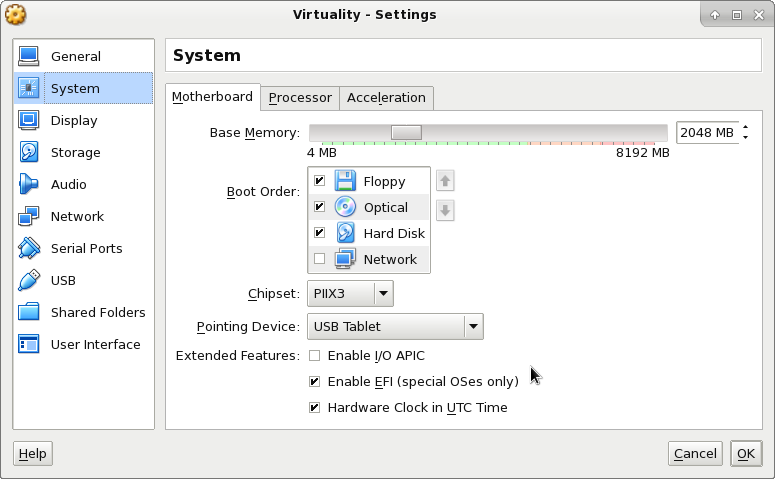
\includegraphics[width=0.6\textwidth]{resin-vbox}
	\caption{Virtualbox general settings for resinOS}
	\label{fig:resingen}
\end{figure}

\begin{figure}
	\centering
	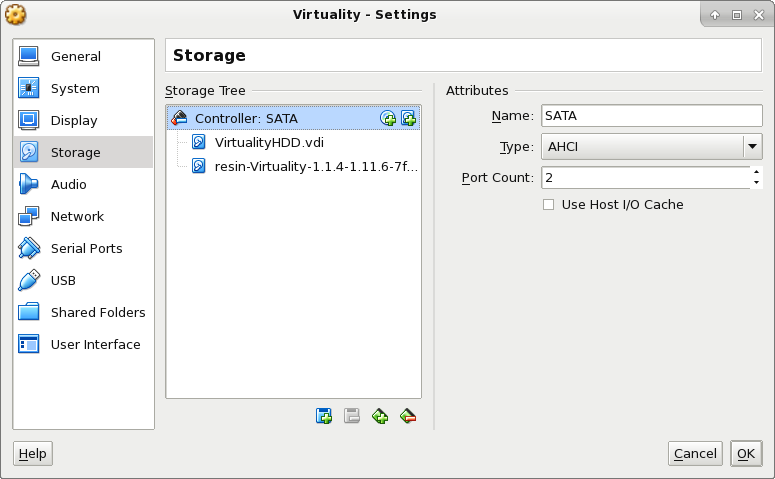
\includegraphics[width=0.6\textwidth]{resin-vbox2}
	\caption{Disk settings for resinOS}
	\label{fig:resindisk}
\end{figure}

To properly connect and download eventual containers we have to configure some forwards. In the ``Network'' menu, select advanced, then Port forward. Configure now the forward of port 8022 to 22  and 2375 to 2375 for client host 10.0.2.15 (usually).

If the virtual machine is run now, the downloaded boot image creates a new instance of resinOS on the previously created virtual drive. The new disk is populates with the settings specified in the configuration step. The system shuts down automatically. Now the resin boot image can be removed.

\subsubsection{Run a Balena container in resinOS}

\textit{resinOS} is shipped with Balena pre-installed and the system is now ready to run any desired container. 
An example application responding to a simple web request can be set-up and tested with the following guide.

Clone the repository to a local directory with
\begin{verbatim}
	git clone https://github.com/resin-io-playground/resinos-sample
\end{verbatim}

now enter the repository and edit ``Dockerfile''. Replace the text after FROM with \textit{resin/intel-nuc-alpine-node:slim}. Now compile and upload the container to the virtual host with

\begin{verbatim}
	sudo resin local push localhost --source .
\end{verbatim}

Browsing to localhost should now display a test page.

\subsection{Ubuntu core}
{\small\textsc{Testrun Ubuntu core, 25/07/18} \bigskip}

\subsubsection{Local Virtual machine}
download and convert kvm image. run as ubunntu. register to ubuntu one. add ssh key for the registration of the ssh in. snaps only in this image. no apt-get. patch not possible as patch command not installed.

Uses snaps for applications

Snap general specifications:
standard in ubuntu since 2 years now (16.04 has them preinstalled)

snap sandboxing
something in between docker and apt
gives the flexibilty of continuous updates of an application without interacting with the filesystem of the client during the installation

has different partitions. The normal filesystem is readonly. The binary section in the image which contains the application is readonly. There is an additional section which is rw where the application can actually write its data. 
The interaction with the system is transparent. no virtual network cards and integration to the x server is seamless. (graphics app are plotted on same screen)
maybe consider snap conversion of apps just to test the outcome. Not a must that the applications are to be on separate sandboxes. -> problem maybe with the portability of the host system, even though fedora ecc also include the snap subsystem

\subsection{Ubuntu Server 16.04.4 with xenomai}

{\small\textsc{Testrun Xenomai, 26/07/18} \bigskip}

\subsubsection{Local Virtual machine}

ubuntu server uses kernel 4.4, thus ideal for kernel 4.9 upgrade

New image, > disk size. uses more than 10gb for kernel compilation. script by pasquale uses older patch name for i-pipe. update the end of the file 4 to 5.

--- corrected folder changes, cd.. was in the wrong position

-> xenomai ! sudo autoreconf
needed as the system and architecture changes

The balena package (one binary) has been installed properly


\subsection{Ubuntu Server 16.04.4 with patch RT}

{\small\textsc{Testrun Preempt-RT, 27/07/18} \bigskip}


\subsubsection{Local Virtual machine}

downloaded patched kernel from kernel.org
make menuconfig
-> (needs libncurses5 libncurses5-dev)

remove cpu-freq and cpu idle (needs PM cpu deactivation first)
search with /

-> need all kernel packages as before
sudo apt-get install git fakeroot build-essential ncurses-dev xz-utils libssl-dev bc
https://medium.freecodecamp.org/building-and-installing-the-latest-linux-kernel-from-source-6d8df5345980

install as in script

\section{Tests of system}

{\small\textsc{Testrun and comparison of systems, 30/07/18} \bigskip}

\subsection{Cyclictest}

apt install xenomai-system-tools

install testbench for realtime
https://wiki.linuxfoundation.org/realtime/documentation/howto/tools/rt-tests#compile-and-instal



./cyclictest 
-n nanosec rtc based
-t num of threads
-l no of loops
-d delay between threads
-p priority of threads
-i interval of thread


example: 
cyclictest -t 50 -i 1000 -d 86400 -l 1000000 -a -p 99 -n

\subsection{Other testing tool}

other tools that might be helpful
htop
iftop
iotop


\section{Additional fixes}

balena, even though installed via script, is not properly configured

https://docs.docker.com/install/linux/linux-postinstall/#configuring-remote-access-with-systemd-unit-file


\section{Issues and verifications}

{\small\textsc{, 31/07/18} \bigskip}



WARN[0001] Your kernel does not support swap memory limit 

Oh nuts, is it...

#CONFIG_MEMCG_SWAP_ENABLED is not set -> WARNING: No swap limit support

and

# CONFIG_MEMCG_KMEM is not set -> WARNING: No memory limit support

possible temporary fix https://github.com/moby/moby/issues/4250



WARN[0001] Your kernel does not support cgroup rt period 
WARN[0001] Your kernel does not support cgroup rt runtime 
-> not activated if Preempt full!!

\section{Virtualization sustainability tests}

{\small\textsc{Testrun Containers \& CPU pinning, 01/08 - 3/08/18} \bigskip}

% AWS ? virtual machine test resoure pinning in vbox -> pin local host? balance share.


man 7 capabilities  -> list of all linux based capabilities


--> check sourcecode of balena tells the compose supported commands and capabilities

creation of a balena container for RT tests


\section{Meetings}

\begin{table}
	\centering
	\caption{List of meetings during the stay at UC Berkeley}
	
	\begin{tabular}{l l l}
	Date & Participants & Topics \\
	\hline
	26/07/18 & Martin Sehr, Ines Ugalde Diaz, Antonio Iannopollo, Florian Hofer & Project setup, generic requirements, questions for BU\\
	31/07/18 & Martin Sehr, Ines Ugalde Diaz, Florian Hofer & Progress of testing, Dummy testing approach\\
	07/08/18 & Ines Ugalde Diaz, Florian Hofer & \\
	10/08/18 & Ines Ugalde Diaz, Florian Hofer & \\
	\hline
	\end{tabular}
	
	\label{tab:meeting}
\end{table}

\end{document}


% Fri Non slide 



